\subsection{Banco de dados relacionais}

\par O modelo de banco de dados relacional foi introduzido em 1970, por Edgar Frank Codd, em uma publicação com o título: “A relational model of data for large shared data banks”, na revista \textit{Association for Computing Machinery} (ACM). Essa publicação demonstrou como tabelas podem ser usadas para representar objetos do mundo real e como os dados podem ser armazenados para os objetos. Neste conceito, a integridade dos dados foi levada mais a sério do que em qualquer modelo de banco de dados antes visto. A partir desta publicação, surgiram muitos bancos de dados que passaram a utilizar este conceito e se tornaram muito utilizados no desenvolvimento de aplicações
\cite{matthew_stones_beginning_databases_with_postgresql}.

\par Segundo \citeonline{matthew_stones_beginning_databases_with_postgresql}, o conceito é baseado na teoria reacional da matemática e por isso há uma grande flexibilidade para o acesso e a manipulação de dados que são gravados no banco. Utilizam-se técnicas simples, como normalização na modelagem do banco de dados, criando várias tabelas relacionadas, que servem como base para consultas usando uma linguagem de consulta quase padronizada, a \textit{Structured Query Language} – SQL\footnotemark[5].

\footnotetext[5]{SQL: \textit{Structured Query Language} - Linguagem para consultas e alterações em bancos de dados.}

% Pode voltar mais a frente no TCC quando for necessário aumentar esta parte
%\par Ainda segundo \citeonline{matthew_stones_beginning_databases_with_postgresql}, um banco de dados relacional contém relações (tabelas) com atributos (colunas) e tuplas (linhas). Todo atributo possui um tipo de dado predefinido, uma tupla representa um conjunto de dados contendo um valor para cada atributo da linha e as tabelas são relacionadas através de chaves.

\par A utilização de banco de dados relacionais geraram a necessidade de dividir os dados agregados utilizados na aplicação em várias relações conforme as regras da normalização. Para recuperar o mesmo dado agregado são necessárias consultas utilizando \textit{joins}\footnotemark[6], uma operação que, dependendo do tamanho das relações e da quantidade de dados, pode não ser tão eficiente. Nos casos em que se precisa obter uma resposta rápida de um sistema, isso se torna uma desvantagem \cite{sadalage_fowler_nosql_distilled_brief_guide}.

\footnotetext[6]{\textit{joins} - função utilizada para realizar a junção entre tabelas, facilitando a busca em bancos de dados relacionais.}

% Pode voltar mais a frente no TCC quando for necessário aumentar esta parte
%\par A figura 6 ilustra bem esta situação de divisão de um agregado e as suas relações resultantes.

% Imagem do exemplo de join - PODE VOLTAR MAIS TARDE NO TCC (Confirmar com o Márcio)
%\begin{figure}[h!]
	%\centerline{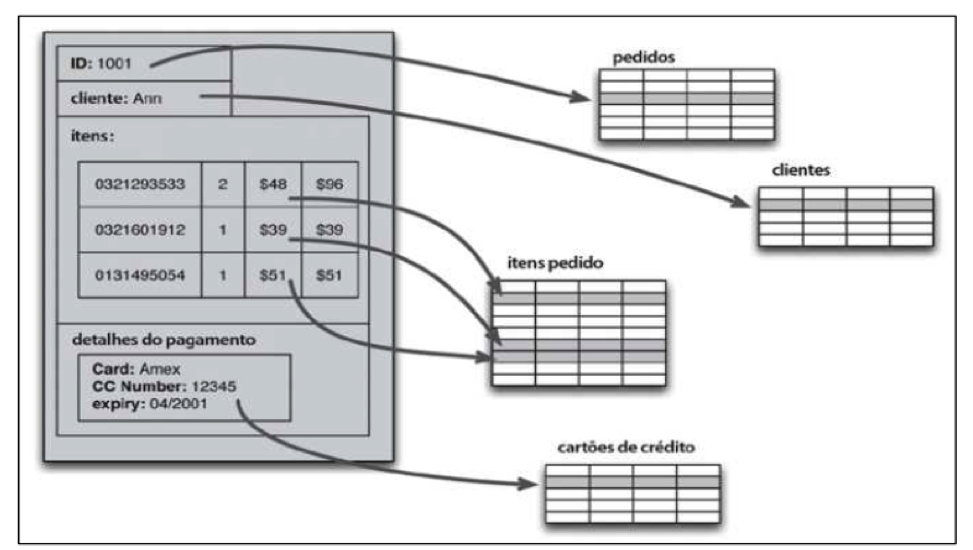
\includegraphics[scale=0.8]{./imagens/example_joins_sadalage.png}}
	%\caption[Agregado no UI é conjunto de várias tuplas de várias tabelas]
	%{Agregado no UI é conjunto de várias tuplas de várias tabelas. \textbf{Fonte:} \citeonline[p. 29]{sadalage_fowler_nosql_distilled_brief_guide}}
	%\label{fig:exemplo1}
%\end{figure}

\par Este foi um dos fatores determinantes que motivaram a criação de novas tecnologias, a fim de sanar o problema mencionado acima. A partir desta motivação, foram desenvolvidos novos modelos de banco de dados, que serão apresentados a seguir.
